\section{Trampoline vs. Hybrid Approach}
\label{sec:trampoline}

\begin{figure}[h!]
  \begin{center}

    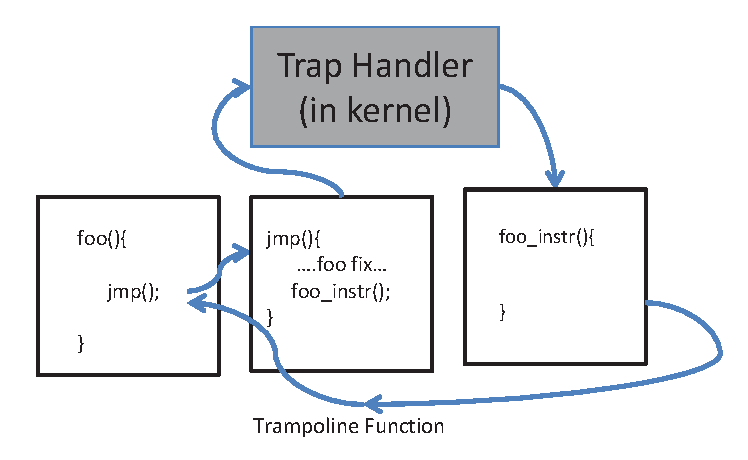
\includegraphics[width=0.95\textwidth]{iprobe/Images/tramp.eps}
    \caption{Traditional Trampoline based Dynamic Instrumentation Mechanisms.}
    \label{fig:tramp}

  \end{center}
\end{figure}

In this section we compare the advantages of our approach compared to traditional trampoline based dynamic instrumentation mechanisms. 
We show the steps followed in trampoline mechanisms, and why our approach has a significant improvement in terms of overhead. 
The basic process of dynamic instrumentation based on trampoline can be divided into 4 steps

\begin{itemize}

\item \textbf{Inspection for Probe Points: } This step inspects and generates a binary patch for the custom instrumentation to be inserted to the target binaries, and find the target probe points which are the code addresses to be modified.

\item \textbf{Memory Allocation for Patching: } Appropriate memory space is allocated for adding the patch and the trampoline code to the target binary.

\item \textbf{Loading and Activation of a Patch: } At run-time the patch is loaded into the target binary, and overwrites the probe point with a jump instruction to a trampoline function and subsequently to the instrumentation function.

\item \textbf{Safety and Reliability Check: } To avoid illegal instructions, it is necessary to check for safety and reliability at the HotPatch stage, and that the logic and correctness of the previous binary remains. 
\end{itemize} 

One of the key reasons for better performance of iProbe as compared to traditional trampoline based designs is the avoidance of multiple jumps enforced in the trampoline mechanism. 
For instance, Figure \ref{fig:tramp} shows the traditional trampoline mechanism used in existing dynamic instrumentation techniques. 
To insert a hook for the function \texttt{foo()}, dynamic instrumentation tools overwrite target probe point instructions with a jump to a small trampoline function (\texttt{jmp()}).
Note that the overwritten code by \texttt{jmp} should be executed somewhere to ensure the correctness of the original program.
The trampoline function executes the overwritten instructions (\texttt{foo fix}) before executing the actual code to be inserted. 
Then this trampoline function in turn makes the call to the instrumentation function (\texttt{foo\_instr}).
Each call instruction can potentially lead to branch mispredictions in the code cache and cause high overhead.
Additionally tools like DTrace, and SystemTap \cite{dtrace,systemtap} have the logger in the kernel space, and cause a context switch in the trampoline using interrupt mechanisms. 

In comparison iProbe has a \texttt{NOP} instruction which can be easily overwritten without resulting in any illegal instructions, and since overwriting is not a problem trampoline function is not required.
This makes the instrumentation process simple resulting in only a single call instruction at all times.

In addition pure binary instrumentation mechanisms need to provide complex guarantees of safety and reliability and hence may lead to further overhead.
Since the patch and trampoline functions overwrite instructions at run-time correctness check must be made at HotPatch time so that an instruction overwrite does not result in an illegal instruction, and that the instructions being patched are not currently being executed.
While this does not enforce a run-time overhead it does enforce a considerable overhead at the HotPatch stage.

Again iProbe avoids this overhead by offloading this process to the compiler stage, and allocating memory ahead of time.


Another important advantage of our hybrid approach as compared to the trampoline approach is that pure dynamic instrumentation techniques are sometimes unable to capture functions from the raw binary. 
This can often be because some compiler optimizations may inherently hide function calls boundaries in the binary. 
A common example of this is \emph{inline functions} where functions are inlined to avoid the creation of a stack frame and concrete calls to these functions. 
This may be done explicitly by the user by defining the function as \emph{inline} or implicitly by the compiler. 
Since our instrumentation uses compiler assisted binary tracing, we are able to use the users definition of functions in the source code to capture entry and exit of functions despite such optimizations.
